% Continuation of Section 4.
\subsection{Sharp frontier-only relaxation loss}

\emph{Economic question.}  What productive value can be lost if compression
preserves the current operating frontier but ignores the capabilities needed
to generate descendants?

Frontier-only pruning replaces the exact constraint \(K_{L'}=K_L\) by
\(F_{L'}=F_L\).  The relaxation is operationally exact today but may remove a
unique module carrier and therefore a positive-mass path to a valuable
descendant.  The bridge construction isolates that loss.

Let
\(L=\{s_0,s_L,s_R,s_M\}\) have frontier
\(F_L=(3,3)\) on two beliefs and closure \(C_L=\{m\}\).  The profiles of
\(s_L\) and \(s_R\) attain the two frontier coordinates, while the dominated
bridge \(s_M\) has profile \((1,1)\) and uniquely carries \(m\).  Hence
\(s_M\) is operationally redundant but generatively essential.  Deleting it
preserves \(F_L\), removes \(m\), and disables the only project leading to
descendant \(c\).

For this canonical one-project comparison, define
\(\operatorname{Loss}_d\) as the retained bridge envelope minus its
frontier-only comparator.  The reward cap \(C\) bounds the complete
distinguished terminal continuation gain, there are no other differential
projects or continuation gains, and the incumbent operating block is common.

\begin{theorem}[Sharp normalized frontier-only relaxation loss]
\label{thm:normalized-frontier-pruning-loss}
Fix exact rationals \(0\le\beta<1\), \(0\le\rho,\pi\le1\), reward cap
\(C\ge0\), cost \(\kappa\ge0\), and delay \(d\ge1\).  Suppose the dominated
bridge uniquely enables a descendant, retention gives survival mass
\(\rho^d\) and admission probability \(\pi\), and deletion makes that
descendant mass zero.  If \(\kappa\le\beta^d\rho^d\pi C\), then
\begin{equation}\label{eq:normalized-pruning-loss}
 \operatorname{Loss}_d
 =\beta^d\rho^d\pi C-\kappa.
\end{equation}
For fixed \((\beta,\rho,\pi,d,\kappa)\), this is the sharp upper bound over
descendant rewards in \([0,C]\), attained at \(C\).  Whenever the denominator
is positive,
\[
 \frac{\operatorname{Loss}_d}
 {\beta^d\rho^d\pi C-\kappa}=1.
\]
Thus the relaxation can destroy the entire attainable net bridge value even
though it leaves the current frontier unchanged.  If \(C\le1\), the additive
loss is at most one; arbitrarily large loss requires reward scaling.
\end{theorem}

The theorem proves an exact and sharp loss statement for the displayed
canonical one-project comparison.  The bridge is operationally redundant
because deleting it preserves \(F_L\), but generatively essential because its
deletion removes \(m\) from \(C_L\) and disables the descendant.  The
normalized loss is one whenever the attainable net bridge value is positive.
This does not assert an unbounded normalized loss: under \(C\le1\) the
additive loss is at most one, and arbitrary additive loss requires the reward
scaling in the corollary below.

Common incumbent operating blocks cancel under frontier equality.  If
operation differs during research, its exact discounted difference must be
added.  The factor \(\rho^d\pi\) comes from the sequential raw generation and
conditional admission rows, not from path--outcome independence.  Finiteness
is used only for the attained one-project maximum; detectability and
contraction are not used.  The catalog and proof are in Appendix~B.

\begin{corollary}[Arbitrary additive loss only by scaling]
\label{thm:scaled-frontier-pruning-loss}
For \(M\in\Q_{\ge0}\), take
\((d,\beta,\rho,\pi,\kappa,C)=(1,1/2,1,1,0,2M)\).  Then
\(\operatorname{Loss}_1=M\).
\end{corollary}

\begin{figure}[ht]
\centering
% Generated by julia/scripts/generate_figure_audit_artifacts.jl.
% Exact source: experiments/results/summaries/innovation_safe_bridge.csv.
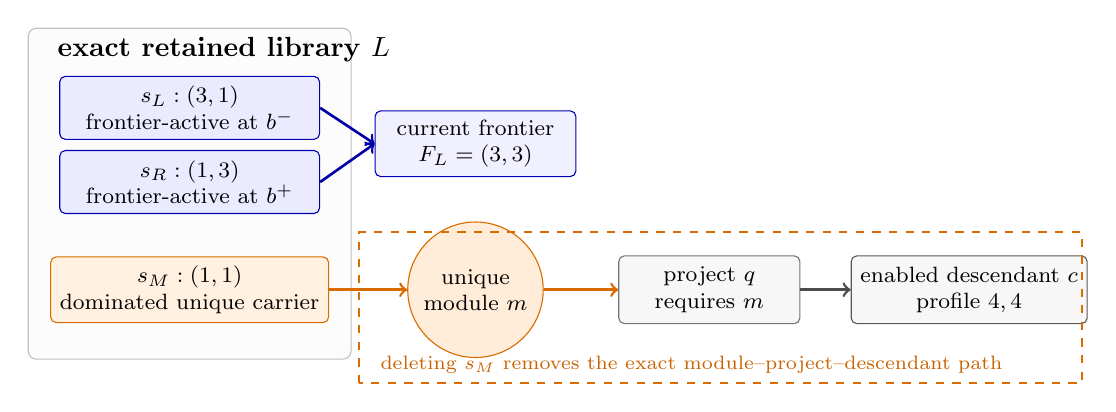
\begin{tikzpicture}[x=1cm,y=0.76cm,font=\footnotesize]
  \tikzset{
    active/.style={draw=blue!70!black,fill=blue!8,rounded corners=2pt,
      minimum width=3.30cm,minimum height=0.80cm,align=center},
    bridge/.style={draw=orange!85!black,fill=orange!12,rounded corners=2pt,
      minimum width=3.30cm,minimum height=0.80cm,align=center},
    module/.style={draw=orange!85!black,fill=orange!15,circle,
      minimum size=1.20cm,align=center},
    project/.style={draw=black!55,fill=black!3,rounded corners=2pt,
      minimum width=2.30cm,minimum height=0.86cm,align=center},
    descendant/.style={draw=black!65,fill=black!3,rounded corners=2pt,
      minimum width=2.50cm,minimum height=0.86cm,align=center},
    flow/.style={->,line width=0.95pt,draw=black!70}
  }
  \draw[draw=black!25,rounded corners=3pt,fill=black!1]
    (-0.2,-0.78) rectangle (3.90,4.75);
  \node[font=\bfseries,anchor=west] at (0.05,4.40)
    {exact retained library \(L\)};

  \node[active] (left) at (1.85,3.42)
    {\(s_L:(3,1)\)\\frontier-active at \(b^-\)};
  \node[active] (right) at (1.85,2.18)
    {\(s_R:(1,3)\)\\frontier-active at \(b^+\)};
  \node[bridge] (bridge) at (1.85,0.38)
    {\(s_M:(1,1)\)\\dominated unique carrier};

  \node[draw=blue!70!black,fill=blue!6,rounded corners=2pt,
    minimum width=2.55cm,minimum height=0.80cm,align=center]
    (frontier) at (5.48,2.82) {current frontier\\\(F_L=(3,3)\)};
  \draw[flow,draw=blue!65!black] (left.east) -- (frontier.west);
  \draw[flow,draw=blue!65!black] (right.east) -- (frontier.west);

  \node[module] (module) at (5.48,0.38) {unique\\module \(m\)};
  \draw[flow,draw=orange!85!black] (bridge.east) -- (module.west);
  \node[project] (project) at (8.45,0.38) {project \(q\)\\requires \(m\)};
  \draw[flow,draw=orange!85!black] (module.east) -- (project.west);
  \node[descendant] (descendant) at (11.75,0.38)
    {enabled descendant \(c\)\\profile \(4,4\)};
  \draw[flow] (project.east) -- (descendant.west);

  \draw[dashed,orange!85!black,line width=0.85pt]
    (4.00,-1.18) rectangle (13.18,1.34);
  \node[anchor=west,text=orange!78!black,font=\scriptsize] at (4.15,-0.87)
    {deleting \(s_M\) removes the exact module--project--descendant path};
\end{tikzpicture}

\caption{Exact bridge-mechanism fixture, not a statistical estimate.  The
frontier-only relaxation deletes the dominated \(s_M\) while preserving the
two-belief frontier \(F_L=(3,3)\), but removes its unique module \(m\),
disables project \(q\), and destroys access to the profile-\((4,4)\)
descendant.  Profiles and dependencies are exact source rows; diagram
coordinates are presentation-only and imply no additional path.}
\label{fig:innovation-safe-bridge}
\end{figure}

\subsection{Capacity-constrained selection}
\label{subsec:resource-statics}

\emph{Economic question.}  If available retention capacity is too small to
preserve a specified source library's productive state, what productive value
is attainable and which outer-certified libraries attain it?

Exact compression starts from a specified source and preserves its productive
state.  Capacity selection instead ranges over the entire finite
outer-certified family \(\mathfrak L_\theta\) and permits productive tradeoffs:
\begin{equation}\label{eq:capacity-value}
 V_\theta^\star(b;B)
 :=\max_{L'\in\mathfrak L_\theta:\,W(L')\le B}V_\theta(b,L').
\end{equation}
The budget is imposed once at retention; it does not alter the raw Bellman
recursion or later admission update.

\begin{theorem}[Finite capacity-constrained retention]
\label{thm:capacity-value}
Suppose \(\mathfrak L_\theta\) contains the zero-burden inactive-only library.
For every \(B\ge0\), the maximum in \eqref{eq:capacity-value} is attained.
If \(B_1\le B_2\), then
\[
 V_\theta^\star(b;B_1)\le V_\theta^\star(b;B_2).
\]
The capacity value is constant between consecutive attainable burdens and can
change only at an attainable burden; every exact forward capacity increment
is nonnegative.  Unit capacity increments need not diminish: an exact
two-module complementarity instance has successive increments \(0\) and \(1\).
\end{theorem}

The theorem proves attainment, monotonicity, and finite step geometry for the
capacity-maximized productive value.  It does not prove uniqueness or
inclusion nesting of capacity maximizers, and it does not imply diminishing
capacity increments: the exact \((0,0,1)\) complementarity profile is the
counterexample.  Discreteness is substantive; an attainable hard-capacity
maximizer may be unsupported by every resource price.

Throughout this theorem and its Lean formalization, the inactive-only library
has burden zero.  Section~6's canonical plots use a separately marked display
translation \(\widetilde W=1+W\); that convention does not change this theorem
or its assumptions.

\subsection{Penalized selection}

\emph{Economic question.}  How does a scalar price on retention burden change
optimized value and the burdens of maximizing outer-certified libraries?

Pricing burden gives the second outer problem
\begin{equation}\label{eq:penalized-value}
 J_\theta^\star(b;\lambda)
 :=\max_{L'\in\mathfrak L_\theta}
 \{V_\theta(b,L')-\lambda W(L')\},
 \qquad \lambda\ge0.
\end{equation}
Each library supplies an affine branch
\(J_{L'}(\lambda)=V_\theta(b,L')-\lambda W(L')\).

\begin{theorem}[Finite penalized value envelope]
\label{thm:penalized-envelope}
For a fixed nonempty finite eligible family, the maximum in
\eqref{eq:penalized-value} is attained.  The optimized value is continuous,
nonincreasing, convex, and piecewise affine in the real price \(\lambda\),
with switching candidates among finitely many pairwise branch intersections.
If \(0\le\lambda_1<\lambda_2\), every optimizer at \(\lambda_2\) has weakly
lower burden than every optimizer at \(\lambda_1\).  Wherever one branch is
strictly dominant, the local slope is \(-W(L')\).
\end{theorem}

The theorem proves the geometry of the optimized penalized-value envelope and
the cross-price order of optimizer burdens.  It orders burdens, not raw
library identities: a higher-price optimizer need not be a sublibrary of a
lower-price optimizer.

For two unequal-burden libraries, their candidate crossing price is
\begin{equation}\label{eq:resource-price-candidate}
 \lambda_{12}
 =\frac{V_\theta(b,L_1)-V_\theta(b,L_2)}
        {W(L_1)-W(L_2)}.
\end{equation}
It is an actual envelope breakpoint only if the two branches both maximize
the penalized objective over the full eligible family there.  Equal-burden
branches are parallel or coincident.  At a tie, the optimizer is set-valued;
the theorem does not assert differentiability at a breakpoint.  Appendix~B
gives the affine-envelope and burden-order arguments.  Online Supplement~S3
records the optional conditional replacement formulation
outside the theorem sequence above.

\subsection{Computational complexity of exact compression}
\label{subsec:aor-safe-compression-complexity}

The exact frontier--closure constraint is directly checkable on a proposed
sublibrary, but finding a minimum-burden feasible sublibrary is not generally
tractable by that fact alone. The following result fixes the finite encoding
and separates the human proof from its executable reduction fixtures.

\begin{theorem}[Identity-closure safe-compression complexity]
\label{thm:aor-safe-compression-complexity}
Consider the finite exact safe-compression decision problem whose input lists
the belief coordinates, rational strategy profiles, positive rational active
weights, module incidences, a mandatory zero-weight inactive strategy,
identity closure, a source library, and a rational burden threshold. Deciding
whether a source sublibrary preserves both the source frontier and source
closure within the threshold is NP-complete, and minimum-weight exact safe
compression is NP-hard. The frontier-only and closure-only decision problems
are each NP-complete. These lower bounds persist under unit active weights.

For identity closure, the combined optimization is exactly weighted hitting
set on the family consisting of every positive-frontier attainer set and every
source-module carrier set. A general-closure problem class containing identity
closure is NP-hard; it is in NP, and hence NP-complete in decision form, when
closure equality is polynomial-time verifiable in the declared encoding.
\end{theorem}

\begin{proof}
Membership in NP follows by using the selected strategy identifiers as a
certificate. Exact rational addition and comparison verify burden in time
polynomial in the listed bit length. At each listed belief, one computes the
candidate maximum and compares it with the source maximum. Under identity
closure, one computes the union of the selected module-incidence rows and
compares it with the source union. Mandatory inactive retention and source
inclusion are direct membership checks.

For hardness, take a set-cover instance with universe \(U\), covering sets
\(A_i\subseteq U\), and positive weights \(w_i\), assuming the listed family
covers \(U\). Create one active strategy \(s_i\) of weight \(w_i\) for each
set. For the closure-only construction, use one belief, give every active
strategy the zero profile, and let \(s_i\) carry exactly the modules indexed by
\(A_i\). The mandatory inactive strategy already preserves the zero frontier,
and a retained library preserves the source identity closure if and only if
the selected sets cover \(U\). Burden is preserved exactly.

For the frontier-only construction, use one belief \(b_u\) for every
\(u\in U\), give \(s_i\) payoff one at \(b_u\) precisely when \(u\in A_i\),
and give every active strategy an empty module row. Because the source family
covers \(U\), its frontier is one at every listed belief. A sublibrary
preserves that frontier if and only if its selected sets cover \(U\), again
with identical burden. Assigning both the incidence profiles and incidence
module rows gives the combined reduction without changing the feasible masks.
The constructors are linear in the explicitly listed incidence matrix.

Weighted set cover therefore transfers NP-hardness and, with membership in NP,
NP-completeness; restricting all weights to one transfers the ordinary
set-cover lower bound. For an arbitrary identity-closure instance, frontier
equality requires selecting at least one source attainer for every belief with
positive source frontier; zero-frontier coordinates are already attained by
the mandatory inactive strategy. Closure equality requires selecting at least
one carrier of every source module. These are exactly the stated hitting-set
obligations. Finally, any general-closure class containing identity closure
inherits the lower bound, while a polynomial closure-equality evaluator adds
the certificate check needed for NP membership.
\end{proof}

This is a human-readable polynomial reduction, not a Lean kernel-verification
claim. The exact Julia constructors independently check weight and feasible-
mask correspondence for the registered fixture and exhaust the declared small
incidence family. Those finite checks validate the implementation of the
reduction; they are not the universal proof above. The theorem supplies no
generic greedy approximation ratio, exchange property, or submodularity
claim.
